% Created by tikzDevice version 0.12.6 on 2026-07-09 15:42:19
% !TEX encoding = UTF-8 Unicode
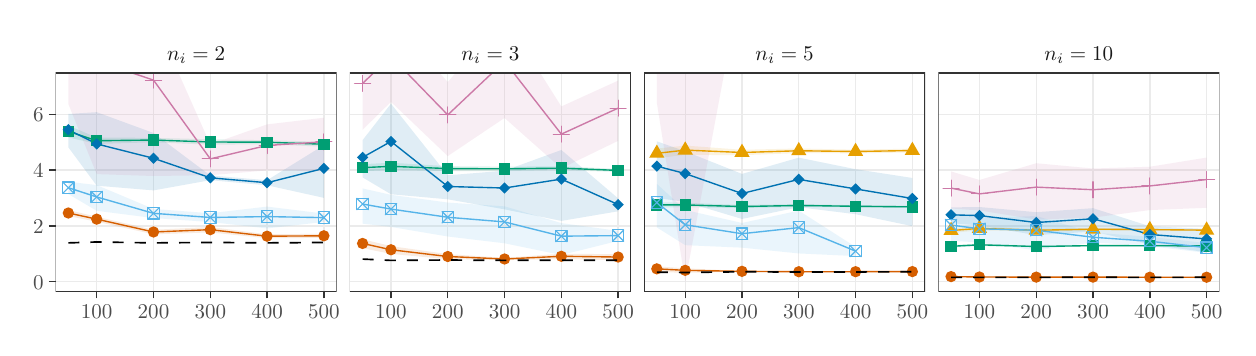
\begin{tikzpicture}[x=1pt,y=1pt]
\definecolor{fillColor}{RGB}{255,255,255}
\path[use as bounding box,fill=fillColor,fill opacity=0.00] (0,0) rectangle (433.62,108.41);
\begin{scope}
\path[clip] (  0.00,  0.00) rectangle (433.62,108.41);
\definecolor{drawColor}{RGB}{255,255,255}
\definecolor{fillColor}{RGB}{255,255,255}

\path[draw=drawColor,line width= 0.5pt,line join=round,line cap=round,fill=fillColor] ( -0.00,  0.00) rectangle (433.62,108.41);
\end{scope}
\begin{scope}
\path[clip] ( 10.07, 12.99) rectangle (111.65, 92.09);
\definecolor{fillColor}{RGB}{255,255,255}

\path[fill=fillColor] ( 10.07, 12.99) rectangle (111.65, 92.09);
\definecolor{drawColor}{gray}{0.92}

\path[draw=drawColor,line width= 0.5pt,line join=round] ( 10.07, 16.58) --
	(111.65, 16.58);

\path[draw=drawColor,line width= 0.5pt,line join=round] ( 10.07, 36.76) --
	(111.65, 36.76);

\path[draw=drawColor,line width= 0.5pt,line join=round] ( 10.07, 56.93) --
	(111.65, 56.93);

\path[draw=drawColor,line width= 0.5pt,line join=round] ( 10.07, 77.10) --
	(111.65, 77.10);

\path[draw=drawColor,line width= 0.5pt,line join=round] ( 24.95, 12.99) --
	( 24.95, 92.09);

\path[draw=drawColor,line width= 0.5pt,line join=round] ( 45.47, 12.99) --
	( 45.47, 92.09);

\path[draw=drawColor,line width= 0.5pt,line join=round] ( 65.99, 12.99) --
	( 65.99, 92.09);

\path[draw=drawColor,line width= 0.5pt,line join=round] ( 86.51, 12.99) --
	( 86.51, 92.09);

\path[draw=drawColor,line width= 0.5pt,line join=round] (107.03, 12.99) --
	(107.03, 92.09);
\definecolor{fillColor}{RGB}{213,94,0}

\path[fill=fillColor,fill opacity=0.12] ( 14.69, 42.51) --
	( 24.95, 40.09) --
	( 45.47, 35.38) --
	( 65.99, 36.37) --
	( 86.51, 33.76) --
	(107.03, 33.92) --
	(107.03, 32.45) --
	( 86.51, 32.33) --
	( 65.99, 34.43) --
	( 45.47, 33.74) --
	( 24.95, 38.31) --
	( 14.69, 40.33) --
	cycle;

\path[] ( 14.69, 42.51) --
	( 24.95, 40.09) --
	( 45.47, 35.38) --
	( 65.99, 36.37) --
	( 86.51, 33.76) --
	(107.03, 33.92);

\path[] (107.03, 32.45) --
	( 86.51, 32.33) --
	( 65.99, 34.43) --
	( 45.47, 33.74) --
	( 24.95, 38.31) --
	( 14.69, 40.33);
\definecolor{fillColor}{RGB}{0,158,115}

\path[fill=fillColor,fill opacity=0.12] ( 14.69, 73.06) --
	( 24.95, 68.70) --
	( 45.47, 68.60) --
	( 65.99, 68.08) --
	( 86.51, 67.74) --
	(107.03, 67.19) --
	(107.03, 65.38) --
	( 86.51, 66.30) --
	( 65.99, 66.11) --
	( 45.47, 67.01) --
	( 24.95, 66.37) --
	( 14.69, 68.74) --
	cycle;

\path[] ( 14.69, 73.06) --
	( 24.95, 68.70) --
	( 45.47, 68.60) --
	( 65.99, 68.08) --
	( 86.51, 67.74) --
	(107.03, 67.19);

\path[] (107.03, 65.38) --
	( 86.51, 66.30) --
	( 65.99, 66.11) --
	( 45.47, 67.01) --
	( 24.95, 66.37) --
	( 14.69, 68.74);
\definecolor{fillColor}{RGB}{0,114,178}

\path[fill=fillColor,fill opacity=0.12] ( 14.69, 77.23) --
	( 24.95, 77.88) --
	( 45.47, 70.36) --
	( 65.99, 55.01) --
	( 86.51, 53.28) --
	(107.03, 65.97) --
	(107.03, 46.92) --
	( 86.51, 51.45) --
	( 65.99, 53.30) --
	( 45.47, 49.61) --
	( 24.95, 51.31) --
	( 14.69, 65.19) --
	cycle;

\path[] ( 14.69, 77.23) --
	( 24.95, 77.88) --
	( 45.47, 70.36) --
	( 65.99, 55.01) --
	( 86.51, 53.28) --
	(107.03, 65.97);

\path[] (107.03, 46.92) --
	( 86.51, 51.45) --
	( 65.99, 53.30) --
	( 45.47, 49.61) --
	( 24.95, 51.31) --
	( 14.69, 65.19);
\definecolor{fillColor}{RGB}{204,121,167}

\path[fill=fillColor,fill opacity=0.12] ( 14.69,115.47) --
	( 24.95,122.46) --
	( 45.47,112.32) --
	( 65.99, 66.21) --
	( 86.51, 73.46) --
	(107.03, 75.86) --
	(107.03, 56.60) --
	( 86.51, 56.83) --
	( 65.99, 55.10) --
	( 45.47, 54.81) --
	( 24.95, 55.50) --
	( 14.69, 80.85) --
	cycle;

\path[] ( 14.69,115.47) --
	( 24.95,122.46) --
	( 45.47,112.32) --
	( 65.99, 66.21) --
	( 86.51, 73.46) --
	(107.03, 75.86);

\path[] (107.03, 56.60) --
	( 86.51, 56.83) --
	( 65.99, 55.10) --
	( 45.47, 54.81) --
	( 24.95, 55.50) --
	( 14.69, 80.85);
\definecolor{fillColor}{RGB}{86,180,233}

\path[fill=fillColor,fill opacity=0.12] ( 14.69, 52.73) --
	( 24.95, 51.53) --
	( 45.47, 42.91) --
	( 65.99, 41.36) --
	( 86.51, 43.75) --
	(107.03, 41.23) --
	(107.03, 38.22) --
	( 86.51, 35.87) --
	( 65.99, 38.19) --
	( 45.47, 39.62) --
	( 24.95, 42.24) --
	( 14.69, 48.29) --
	cycle;

\path[] ( 14.69, 52.73) --
	( 24.95, 51.53) --
	( 45.47, 42.91) --
	( 65.99, 41.36) --
	( 86.51, 43.75) --
	(107.03, 41.23);

\path[] (107.03, 38.22) --
	( 86.51, 35.87) --
	( 65.99, 38.19) --
	( 45.47, 39.62) --
	( 24.95, 42.24) --
	( 14.69, 48.29);
\definecolor{drawColor}{RGB}{213,94,0}

\path[draw=drawColor,line width= 0.5pt,line join=round] ( 14.69, 41.44) --
	( 24.95, 39.22) --
	( 45.47, 34.58) --
	( 65.99, 35.42) --
	( 86.51, 33.06) --
	(107.03, 33.20);
\definecolor{drawColor}{RGB}{0,158,115}

\path[draw=drawColor,line width= 0.5pt,line join=round] ( 14.69, 70.94) --
	( 24.95, 67.55) --
	( 45.47, 67.81) --
	( 65.99, 67.10) --
	( 86.51, 67.02) --
	(107.03, 66.29);
\definecolor{drawColor}{RGB}{0,114,178}

\path[draw=drawColor,line width= 0.5pt,line join=round] ( 14.69, 71.54) --
	( 24.95, 66.40) --
	( 45.47, 61.21) --
	( 65.99, 54.16) --
	( 86.51, 52.38) --
	(107.03, 57.57);
\definecolor{drawColor}{RGB}{204,121,167}

\path[draw=drawColor,line width= 0.5pt,line join=round] ( 14.69, 99.97) --
	( 24.95, 96.35) --
	( 45.47, 89.47) --
	( 65.99, 61.00) --
	( 86.51, 65.85) --
	(107.03, 67.15);
\definecolor{drawColor}{RGB}{86,180,233}

\path[draw=drawColor,line width= 0.5pt,line join=round] ( 14.69, 50.58) --
	( 24.95, 47.24) --
	( 45.47, 41.32) --
	( 65.99, 39.83) --
	( 86.51, 40.14) --
	(107.03, 39.77);
\definecolor{fillColor}{RGB}{213,94,0}

\path[fill=fillColor] ( 14.69, 41.44) circle (  2.05);
\definecolor{drawColor}{RGB}{204,121,167}

\path[draw=drawColor,line width= 0.4pt,line join=round,line cap=round] ( 11.79, 99.97) -- ( 17.59, 99.97);

\path[draw=drawColor,line width= 0.4pt,line join=round,line cap=round] ( 14.69, 97.07) -- ( 14.69,102.88);
\definecolor{fillColor}{RGB}{0,158,115}

\path[fill=fillColor] ( 12.64, 68.89) --
	( 16.74, 68.89) --
	( 16.74, 72.99) --
	( 12.64, 72.99) --
	cycle;
\definecolor{fillColor}{RGB}{0,114,178}

\path[fill=fillColor] ( 12.64, 71.54) --
	( 14.69, 73.59) --
	( 16.74, 71.54) --
	( 14.69, 69.49) --
	cycle;
\definecolor{drawColor}{RGB}{86,180,233}

\path[draw=drawColor,line width= 0.4pt,line join=round,line cap=round] ( 12.64, 48.53) rectangle ( 16.74, 52.63);

\path[draw=drawColor,line width= 0.4pt,line join=round,line cap=round] ( 12.64, 48.53) -- ( 16.74, 52.63);

\path[draw=drawColor,line width= 0.4pt,line join=round,line cap=round] ( 12.64, 52.63) -- ( 16.74, 48.53);
\definecolor{fillColor}{RGB}{213,94,0}

\path[fill=fillColor] ( 24.95, 39.22) circle (  2.05);
\definecolor{drawColor}{RGB}{204,121,167}

\path[draw=drawColor,line width= 0.4pt,line join=round,line cap=round] ( 22.05, 96.35) -- ( 27.85, 96.35);

\path[draw=drawColor,line width= 0.4pt,line join=round,line cap=round] ( 24.95, 93.45) -- ( 24.95, 99.25);
\definecolor{fillColor}{RGB}{0,158,115}

\path[fill=fillColor] ( 22.90, 65.50) --
	( 27.00, 65.50) --
	( 27.00, 69.60) --
	( 22.90, 69.60) --
	cycle;
\definecolor{fillColor}{RGB}{0,114,178}

\path[fill=fillColor] ( 22.90, 66.40) --
	( 24.95, 68.45) --
	( 27.00, 66.40) --
	( 24.95, 64.35) --
	cycle;
\definecolor{drawColor}{RGB}{86,180,233}

\path[draw=drawColor,line width= 0.4pt,line join=round,line cap=round] ( 22.90, 45.19) rectangle ( 27.00, 49.29);

\path[draw=drawColor,line width= 0.4pt,line join=round,line cap=round] ( 22.90, 45.19) -- ( 27.00, 49.29);

\path[draw=drawColor,line width= 0.4pt,line join=round,line cap=round] ( 22.90, 49.29) -- ( 27.00, 45.19);
\definecolor{fillColor}{RGB}{213,94,0}

\path[fill=fillColor] ( 45.47, 34.58) circle (  2.05);
\definecolor{drawColor}{RGB}{204,121,167}

\path[draw=drawColor,line width= 0.4pt,line join=round,line cap=round] ( 42.57, 89.47) -- ( 48.37, 89.47);

\path[draw=drawColor,line width= 0.4pt,line join=round,line cap=round] ( 45.47, 86.57) -- ( 45.47, 92.38);
\definecolor{fillColor}{RGB}{0,158,115}

\path[fill=fillColor] ( 43.42, 65.76) --
	( 47.52, 65.76) --
	( 47.52, 69.86) --
	( 43.42, 69.86) --
	cycle;
\definecolor{fillColor}{RGB}{0,114,178}

\path[fill=fillColor] ( 43.42, 61.21) --
	( 45.47, 63.26) --
	( 47.52, 61.21) --
	( 45.47, 59.16) --
	cycle;
\definecolor{drawColor}{RGB}{86,180,233}

\path[draw=drawColor,line width= 0.4pt,line join=round,line cap=round] ( 43.42, 39.27) rectangle ( 47.52, 43.37);

\path[draw=drawColor,line width= 0.4pt,line join=round,line cap=round] ( 43.42, 39.27) -- ( 47.52, 43.37);

\path[draw=drawColor,line width= 0.4pt,line join=round,line cap=round] ( 43.42, 43.37) -- ( 47.52, 39.27);
\definecolor{fillColor}{RGB}{213,94,0}

\path[fill=fillColor] ( 65.99, 35.42) circle (  2.05);
\definecolor{drawColor}{RGB}{204,121,167}

\path[draw=drawColor,line width= 0.4pt,line join=round,line cap=round] ( 63.09, 61.00) -- ( 68.89, 61.00);

\path[draw=drawColor,line width= 0.4pt,line join=round,line cap=round] ( 65.99, 58.10) -- ( 65.99, 63.90);
\definecolor{fillColor}{RGB}{0,158,115}

\path[fill=fillColor] ( 63.94, 65.05) --
	( 68.04, 65.05) --
	( 68.04, 69.15) --
	( 63.94, 69.15) --
	cycle;
\definecolor{fillColor}{RGB}{0,114,178}

\path[fill=fillColor] ( 63.94, 54.16) --
	( 65.99, 56.22) --
	( 68.04, 54.16) --
	( 65.99, 52.11) --
	cycle;
\definecolor{drawColor}{RGB}{86,180,233}

\path[draw=drawColor,line width= 0.4pt,line join=round,line cap=round] ( 63.94, 37.78) rectangle ( 68.04, 41.88);

\path[draw=drawColor,line width= 0.4pt,line join=round,line cap=round] ( 63.94, 37.78) -- ( 68.04, 41.88);

\path[draw=drawColor,line width= 0.4pt,line join=round,line cap=round] ( 63.94, 41.88) -- ( 68.04, 37.78);
\definecolor{fillColor}{RGB}{213,94,0}

\path[fill=fillColor] ( 86.51, 33.06) circle (  2.05);
\definecolor{drawColor}{RGB}{204,121,167}

\path[draw=drawColor,line width= 0.4pt,line join=round,line cap=round] ( 83.61, 65.85) -- ( 89.41, 65.85);

\path[draw=drawColor,line width= 0.4pt,line join=round,line cap=round] ( 86.51, 62.95) -- ( 86.51, 68.75);
\definecolor{fillColor}{RGB}{0,158,115}

\path[fill=fillColor] ( 84.46, 64.97) --
	( 88.56, 64.97) --
	( 88.56, 69.08) --
	( 84.46, 69.08) --
	cycle;
\definecolor{fillColor}{RGB}{0,114,178}

\path[fill=fillColor] ( 84.46, 52.38) --
	( 86.51, 54.43) --
	( 88.56, 52.38) --
	( 86.51, 50.33) --
	cycle;
\definecolor{drawColor}{RGB}{86,180,233}

\path[draw=drawColor,line width= 0.4pt,line join=round,line cap=round] ( 84.46, 38.09) rectangle ( 88.56, 42.19);

\path[draw=drawColor,line width= 0.4pt,line join=round,line cap=round] ( 84.46, 38.09) -- ( 88.56, 42.19);

\path[draw=drawColor,line width= 0.4pt,line join=round,line cap=round] ( 84.46, 42.19) -- ( 88.56, 38.09);
\definecolor{fillColor}{RGB}{213,94,0}

\path[fill=fillColor] (107.03, 33.20) circle (  2.05);
\definecolor{drawColor}{RGB}{204,121,167}

\path[draw=drawColor,line width= 0.4pt,line join=round,line cap=round] (104.13, 67.15) -- (109.93, 67.15);

\path[draw=drawColor,line width= 0.4pt,line join=round,line cap=round] (107.03, 64.25) -- (107.03, 70.05);
\definecolor{fillColor}{RGB}{0,158,115}

\path[fill=fillColor] (104.98, 64.24) --
	(109.08, 64.24) --
	(109.08, 68.34) --
	(104.98, 68.34) --
	cycle;
\definecolor{fillColor}{RGB}{0,114,178}

\path[fill=fillColor] (104.98, 57.57) --
	(107.03, 59.62) --
	(109.08, 57.57) --
	(107.03, 55.51) --
	cycle;
\definecolor{drawColor}{RGB}{86,180,233}

\path[draw=drawColor,line width= 0.4pt,line join=round,line cap=round] (104.98, 37.72) rectangle (109.08, 41.83);

\path[draw=drawColor,line width= 0.4pt,line join=round,line cap=round] (104.98, 37.72) -- (109.08, 41.83);

\path[draw=drawColor,line width= 0.4pt,line join=round,line cap=round] (104.98, 41.83) -- (109.08, 37.72);
\definecolor{drawColor}{RGB}{0,0,0}

\path[draw=drawColor,line width= 0.6pt,dash pattern=on 4pt off 4pt ,line join=round] ( 14.69, 30.64) --
	( 24.95, 30.97) --
	( 45.47, 30.64) --
	( 65.99, 30.81) --
	( 86.51, 30.65) --
	(107.03, 30.78);
\definecolor{drawColor}{gray}{0.20}

\path[draw=drawColor,line width= 0.5pt,line join=round,line cap=round] ( 10.07, 12.99) rectangle (111.65, 92.09);
\end{scope}
\begin{scope}
\path[clip] (116.40, 12.99) rectangle (217.97, 92.09);
\definecolor{fillColor}{RGB}{255,255,255}

\path[fill=fillColor] (116.40, 12.99) rectangle (217.97, 92.09);
\definecolor{drawColor}{gray}{0.92}

\path[draw=drawColor,line width= 0.5pt,line join=round] (116.40, 16.58) --
	(217.97, 16.58);

\path[draw=drawColor,line width= 0.5pt,line join=round] (116.40, 36.76) --
	(217.97, 36.76);

\path[draw=drawColor,line width= 0.5pt,line join=round] (116.40, 56.93) --
	(217.97, 56.93);

\path[draw=drawColor,line width= 0.5pt,line join=round] (116.40, 77.10) --
	(217.97, 77.10);

\path[draw=drawColor,line width= 0.5pt,line join=round] (131.28, 12.99) --
	(131.28, 92.09);

\path[draw=drawColor,line width= 0.5pt,line join=round] (151.80, 12.99) --
	(151.80, 92.09);

\path[draw=drawColor,line width= 0.5pt,line join=round] (172.32, 12.99) --
	(172.32, 92.09);

\path[draw=drawColor,line width= 0.5pt,line join=round] (192.84, 12.99) --
	(192.84, 92.09);

\path[draw=drawColor,line width= 0.5pt,line join=round] (213.36, 12.99) --
	(213.36, 92.09);
\definecolor{fillColor}{RGB}{213,94,0}

\path[fill=fillColor,fill opacity=0.12] (121.02, 31.97) --
	(131.28, 29.47) --
	(151.80, 26.59) --
	(172.32, 25.22) --
	(192.84, 26.73) --
	(213.36, 26.55) --
	(213.36, 24.37) --
	(192.84, 24.77) --
	(172.32, 24.40) --
	(151.80, 24.76) --
	(131.28, 26.67) --
	(121.02, 28.73) --
	cycle;

\path[] (121.02, 31.97) --
	(131.28, 29.47) --
	(151.80, 26.59) --
	(172.32, 25.22) --
	(192.84, 26.73) --
	(213.36, 26.55);

\path[] (213.36, 24.37) --
	(192.84, 24.77) --
	(172.32, 24.40) --
	(151.80, 24.76) --
	(131.28, 26.67) --
	(121.02, 28.73);
\definecolor{fillColor}{RGB}{0,158,115}

\path[fill=fillColor,fill opacity=0.12] (121.02, 59.08) --
	(131.28, 59.60) --
	(151.80, 58.37) --
	(172.32, 58.20) --
	(192.84, 58.31) --
	(213.36, 57.39) --
	(213.36, 56.25) --
	(192.84, 56.99) --
	(172.32, 56.59) --
	(151.80, 56.62) --
	(131.28, 56.95) --
	(121.02, 56.54) --
	cycle;

\path[] (121.02, 59.08) --
	(131.28, 59.60) --
	(151.80, 58.37) --
	(172.32, 58.20) --
	(192.84, 58.31) --
	(213.36, 57.39);

\path[] (213.36, 56.25) --
	(192.84, 56.99) --
	(172.32, 56.59) --
	(151.80, 56.62) --
	(131.28, 56.95) --
	(121.02, 56.54);
\definecolor{fillColor}{RGB}{0,114,178}

\path[fill=fillColor,fill opacity=0.12] (121.02, 67.76) --
	(131.28, 80.94) --
	(151.80, 55.07) --
	(172.32, 56.72) --
	(192.84, 64.22) --
	(213.36, 46.73) --
	(213.36, 42.06) --
	(192.84, 38.58) --
	(172.32, 42.76) --
	(151.80, 46.39) --
	(131.28, 48.22) --
	(121.02, 54.31) --
	cycle;

\path[] (121.02, 67.76) --
	(131.28, 80.94) --
	(151.80, 55.07) --
	(172.32, 56.72) --
	(192.84, 64.22) --
	(213.36, 46.73);

\path[] (213.36, 42.06) --
	(192.84, 38.58) --
	(172.32, 42.76) --
	(151.80, 46.39) --
	(131.28, 48.22) --
	(121.02, 54.31);
\definecolor{fillColor}{RGB}{204,121,167}

\path[fill=fillColor,fill opacity=0.12] (121.02,101.81) --
	(131.28,111.62) --
	(151.80, 88.76) --
	(172.32,112.45) --
	(192.84, 79.94) --
	(213.36, 89.27) --
	(213.36, 67.52) --
	(192.84, 57.57) --
	(172.32, 75.79) --
	(151.80, 62.01) --
	(131.28, 81.60) --
	(121.02, 71.52) --
	cycle;

\path[] (121.02,101.81) --
	(131.28,111.62) --
	(151.80, 88.76) --
	(172.32,112.45) --
	(192.84, 79.94) --
	(213.36, 89.27);

\path[] (213.36, 67.52) --
	(192.84, 57.57) --
	(172.32, 75.79) --
	(151.80, 62.01) --
	(131.28, 81.60) --
	(121.02, 71.52);
\definecolor{fillColor}{RGB}{86,180,233}

\path[fill=fillColor,fill opacity=0.12] (121.02, 50.31) --
	(131.28, 48.01) --
	(151.80, 45.21) --
	(172.32, 43.84) --
	(192.84, 37.79) --
	(213.36, 34.97) --
	(213.36, 31.36) --
	(192.84, 26.26) --
	(172.32, 30.50) --
	(151.80, 32.95) --
	(131.28, 36.41) --
	(121.02, 37.59) --
	cycle;

\path[] (121.02, 50.31) --
	(131.28, 48.01) --
	(151.80, 45.21) --
	(172.32, 43.84) --
	(192.84, 37.79) --
	(213.36, 34.97);

\path[] (213.36, 31.36) --
	(192.84, 26.26) --
	(172.32, 30.50) --
	(151.80, 32.95) --
	(131.28, 36.41) --
	(121.02, 37.59);
\definecolor{drawColor}{RGB}{213,94,0}

\path[draw=drawColor,line width= 0.5pt,line join=round] (121.02, 30.44) --
	(131.28, 28.16) --
	(151.80, 25.72) --
	(172.32, 24.82) --
	(192.84, 25.80) --
	(213.36, 25.53);
\definecolor{drawColor}{RGB}{0,158,115}

\path[draw=drawColor,line width= 0.5pt,line join=round] (121.02, 57.83) --
	(131.28, 58.30) --
	(151.80, 57.50) --
	(172.32, 57.41) --
	(192.84, 57.65) --
	(213.36, 56.83);
\definecolor{drawColor}{RGB}{0,114,178}

\path[draw=drawColor,line width= 0.5pt,line join=round] (121.02, 61.54) --
	(131.28, 67.29) --
	(151.80, 51.01) --
	(172.32, 50.47) --
	(192.84, 53.69) --
	(213.36, 44.49);
\definecolor{drawColor}{RGB}{204,121,167}

\path[draw=drawColor,line width= 0.5pt,line join=round] (121.02, 88.28) --
	(131.28, 98.00) --
	(151.80, 76.89) --
	(172.32, 96.26) --
	(192.84, 69.94) --
	(213.36, 79.34);
\definecolor{drawColor}{RGB}{86,180,233}

\path[draw=drawColor,line width= 0.5pt,line join=round] (121.02, 44.68) --
	(131.28, 42.86) --
	(151.80, 39.90) --
	(172.32, 38.22) --
	(192.84, 33.07) --
	(213.36, 33.27);
\definecolor{fillColor}{RGB}{213,94,0}

\path[fill=fillColor] (121.02, 30.44) circle (  2.05);
\definecolor{drawColor}{RGB}{204,121,167}

\path[draw=drawColor,line width= 0.4pt,line join=round,line cap=round] (118.11, 88.28) -- (123.92, 88.28);

\path[draw=drawColor,line width= 0.4pt,line join=round,line cap=round] (121.02, 85.38) -- (121.02, 91.18);
\definecolor{fillColor}{RGB}{0,158,115}

\path[fill=fillColor] (118.96, 55.78) --
	(123.07, 55.78) --
	(123.07, 59.88) --
	(118.96, 59.88) --
	cycle;
\definecolor{fillColor}{RGB}{0,114,178}

\path[fill=fillColor] (118.96, 61.54) --
	(121.02, 63.59) --
	(123.07, 61.54) --
	(121.02, 59.49) --
	cycle;
\definecolor{drawColor}{RGB}{86,180,233}

\path[draw=drawColor,line width= 0.4pt,line join=round,line cap=round] (118.96, 42.63) rectangle (123.07, 46.73);

\path[draw=drawColor,line width= 0.4pt,line join=round,line cap=round] (118.96, 42.63) -- (123.07, 46.73);

\path[draw=drawColor,line width= 0.4pt,line join=round,line cap=round] (118.96, 46.73) -- (123.07, 42.63);
\definecolor{fillColor}{RGB}{213,94,0}

\path[fill=fillColor] (131.28, 28.16) circle (  2.05);
\definecolor{drawColor}{RGB}{204,121,167}

\path[draw=drawColor,line width= 0.4pt,line join=round,line cap=round] (128.37, 98.00) -- (134.18, 98.00);

\path[draw=drawColor,line width= 0.4pt,line join=round,line cap=round] (131.28, 95.10) -- (131.28,100.91);
\definecolor{fillColor}{RGB}{0,158,115}

\path[fill=fillColor] (129.22, 56.24) --
	(133.33, 56.24) --
	(133.33, 60.35) --
	(129.22, 60.35) --
	cycle;
\definecolor{fillColor}{RGB}{0,114,178}

\path[fill=fillColor] (129.22, 67.29) --
	(131.28, 69.34) --
	(133.33, 67.29) --
	(131.28, 65.24) --
	cycle;
\definecolor{drawColor}{RGB}{86,180,233}

\path[draw=drawColor,line width= 0.4pt,line join=round,line cap=round] (129.22, 40.81) rectangle (133.33, 44.91);

\path[draw=drawColor,line width= 0.4pt,line join=round,line cap=round] (129.22, 40.81) -- (133.33, 44.91);

\path[draw=drawColor,line width= 0.4pt,line join=round,line cap=round] (129.22, 44.91) -- (133.33, 40.81);
\definecolor{fillColor}{RGB}{213,94,0}

\path[fill=fillColor] (151.80, 25.72) circle (  2.05);
\definecolor{drawColor}{RGB}{204,121,167}

\path[draw=drawColor,line width= 0.4pt,line join=round,line cap=round] (148.89, 76.89) -- (154.70, 76.89);

\path[draw=drawColor,line width= 0.4pt,line join=round,line cap=round] (151.80, 73.98) -- (151.80, 79.79);
\definecolor{fillColor}{RGB}{0,158,115}

\path[fill=fillColor] (149.74, 55.45) --
	(153.85, 55.45) --
	(153.85, 59.56) --
	(149.74, 59.56) --
	cycle;
\definecolor{fillColor}{RGB}{0,114,178}

\path[fill=fillColor] (149.74, 51.01) --
	(151.80, 53.06) --
	(153.85, 51.01) --
	(151.80, 48.95) --
	cycle;
\definecolor{drawColor}{RGB}{86,180,233}

\path[draw=drawColor,line width= 0.4pt,line join=round,line cap=round] (149.74, 37.85) rectangle (153.85, 41.95);

\path[draw=drawColor,line width= 0.4pt,line join=round,line cap=round] (149.74, 37.85) -- (153.85, 41.95);

\path[draw=drawColor,line width= 0.4pt,line join=round,line cap=round] (149.74, 41.95) -- (153.85, 37.85);
\definecolor{fillColor}{RGB}{213,94,0}

\path[fill=fillColor] (172.32, 24.82) circle (  2.05);
\definecolor{drawColor}{RGB}{204,121,167}

\path[draw=drawColor,line width= 0.4pt,line join=round,line cap=round] (169.41, 96.26) -- (175.22, 96.26);

\path[draw=drawColor,line width= 0.4pt,line join=round,line cap=round] (172.32, 93.36) -- (172.32, 99.16);
\definecolor{fillColor}{RGB}{0,158,115}

\path[fill=fillColor] (170.26, 55.35) --
	(174.37, 55.35) --
	(174.37, 59.46) --
	(170.26, 59.46) --
	cycle;
\definecolor{fillColor}{RGB}{0,114,178}

\path[fill=fillColor] (170.26, 50.47) --
	(172.32, 52.52) --
	(174.37, 50.47) --
	(172.32, 48.42) --
	cycle;
\definecolor{drawColor}{RGB}{86,180,233}

\path[draw=drawColor,line width= 0.4pt,line join=round,line cap=round] (170.26, 36.17) rectangle (174.37, 40.28);

\path[draw=drawColor,line width= 0.4pt,line join=round,line cap=round] (170.26, 36.17) -- (174.37, 40.28);

\path[draw=drawColor,line width= 0.4pt,line join=round,line cap=round] (170.26, 40.28) -- (174.37, 36.17);
\definecolor{fillColor}{RGB}{213,94,0}

\path[fill=fillColor] (192.84, 25.80) circle (  2.05);
\definecolor{drawColor}{RGB}{204,121,167}

\path[draw=drawColor,line width= 0.4pt,line join=round,line cap=round] (189.93, 69.94) -- (195.74, 69.94);

\path[draw=drawColor,line width= 0.4pt,line join=round,line cap=round] (192.84, 67.04) -- (192.84, 72.84);
\definecolor{fillColor}{RGB}{0,158,115}

\path[fill=fillColor] (190.78, 55.60) --
	(194.89, 55.60) --
	(194.89, 59.71) --
	(190.78, 59.71) --
	cycle;
\definecolor{fillColor}{RGB}{0,114,178}

\path[fill=fillColor] (190.78, 53.69) --
	(192.84, 55.74) --
	(194.89, 53.69) --
	(192.84, 51.64) --
	cycle;
\definecolor{drawColor}{RGB}{86,180,233}

\path[draw=drawColor,line width= 0.4pt,line join=round,line cap=round] (190.78, 31.02) rectangle (194.89, 35.12);

\path[draw=drawColor,line width= 0.4pt,line join=round,line cap=round] (190.78, 31.02) -- (194.89, 35.12);

\path[draw=drawColor,line width= 0.4pt,line join=round,line cap=round] (190.78, 35.12) -- (194.89, 31.02);
\definecolor{fillColor}{RGB}{213,94,0}

\path[fill=fillColor] (213.36, 25.53) circle (  2.05);
\definecolor{drawColor}{RGB}{204,121,167}

\path[draw=drawColor,line width= 0.4pt,line join=round,line cap=round] (210.45, 79.34) -- (216.26, 79.34);

\path[draw=drawColor,line width= 0.4pt,line join=round,line cap=round] (213.36, 76.44) -- (213.36, 82.24);
\definecolor{fillColor}{RGB}{0,158,115}

\path[fill=fillColor] (211.30, 54.78) --
	(215.41, 54.78) --
	(215.41, 58.88) --
	(211.30, 58.88) --
	cycle;
\definecolor{fillColor}{RGB}{0,114,178}

\path[fill=fillColor] (211.30, 44.49) --
	(213.36, 46.54) --
	(215.41, 44.49) --
	(213.36, 42.44) --
	cycle;
\definecolor{drawColor}{RGB}{86,180,233}

\path[draw=drawColor,line width= 0.4pt,line join=round,line cap=round] (211.30, 31.21) rectangle (215.41, 35.32);

\path[draw=drawColor,line width= 0.4pt,line join=round,line cap=round] (211.30, 31.21) -- (215.41, 35.32);

\path[draw=drawColor,line width= 0.4pt,line join=round,line cap=round] (211.30, 35.32) -- (215.41, 31.21);
\definecolor{drawColor}{RGB}{0,0,0}

\path[draw=drawColor,line width= 0.6pt,dash pattern=on 4pt off 4pt ,line join=round] (121.02, 24.79) --
	(131.28, 24.31) --
	(151.80, 24.45) --
	(172.32, 24.33) --
	(192.84, 24.39) --
	(213.36, 24.36);
\definecolor{drawColor}{gray}{0.20}

\path[draw=drawColor,line width= 0.5pt,line join=round,line cap=round] (116.40, 12.99) rectangle (217.97, 92.09);
\end{scope}
\begin{scope}
\path[clip] (222.72, 12.99) rectangle (324.30, 92.09);
\definecolor{fillColor}{RGB}{255,255,255}

\path[fill=fillColor] (222.72, 12.99) rectangle (324.30, 92.09);
\definecolor{drawColor}{gray}{0.92}

\path[draw=drawColor,line width= 0.5pt,line join=round] (222.72, 16.58) --
	(324.30, 16.58);

\path[draw=drawColor,line width= 0.5pt,line join=round] (222.72, 36.76) --
	(324.30, 36.76);

\path[draw=drawColor,line width= 0.5pt,line join=round] (222.72, 56.93) --
	(324.30, 56.93);

\path[draw=drawColor,line width= 0.5pt,line join=round] (222.72, 77.10) --
	(324.30, 77.10);

\path[draw=drawColor,line width= 0.5pt,line join=round] (237.60, 12.99) --
	(237.60, 92.09);

\path[draw=drawColor,line width= 0.5pt,line join=round] (258.12, 12.99) --
	(258.12, 92.09);

\path[draw=drawColor,line width= 0.5pt,line join=round] (278.64, 12.99) --
	(278.64, 92.09);

\path[draw=drawColor,line width= 0.5pt,line join=round] (299.16, 12.99) --
	(299.16, 92.09);

\path[draw=drawColor,line width= 0.5pt,line join=round] (319.68, 12.99) --
	(319.68, 92.09);
\definecolor{fillColor}{RGB}{213,94,0}

\path[fill=fillColor,fill opacity=0.12] (227.34, 22.16) --
	(237.60, 21.45) --
	(258.12, 20.49) --
	(278.64, 20.31) --
	(299.16, 20.31) --
	(319.68, 20.37) --
	(319.68, 20.18) --
	(299.16, 20.13) --
	(278.64, 20.11) --
	(258.12, 20.23) --
	(237.60, 19.82) --
	(227.34, 20.13) --
	cycle;

\path[] (227.34, 22.16) --
	(237.60, 21.45) --
	(258.12, 20.49) --
	(278.64, 20.31) --
	(299.16, 20.31) --
	(319.68, 20.37);

\path[] (319.68, 20.18) --
	(299.16, 20.13) --
	(278.64, 20.11) --
	(258.12, 20.23) --
	(237.60, 19.82) --
	(227.34, 20.13);
\definecolor{fillColor}{RGB}{230,159,0}

\path[fill=fillColor,fill opacity=0.12] (227.34, 64.71) --
	(237.60, 65.81) --
	(258.12, 64.28) --
	(278.64, 64.75) --
	(299.16, 64.31) --
	(319.68, 64.70) --
	(319.68, 63.32) --
	(299.16, 63.01) --
	(278.64, 63.09) --
	(258.12, 62.33) --
	(237.60, 62.46) --
	(227.34, 61.22) --
	cycle;

\path[] (227.34, 64.71) --
	(237.60, 65.81) --
	(258.12, 64.28) --
	(278.64, 64.75) --
	(299.16, 64.31) --
	(319.68, 64.70);

\path[] (319.68, 63.32) --
	(299.16, 63.01) --
	(278.64, 63.09) --
	(258.12, 62.33) --
	(237.60, 62.46) --
	(227.34, 61.22);
\definecolor{fillColor}{RGB}{0,158,115}

\path[fill=fillColor,fill opacity=0.12] (227.34, 45.36) --
	(237.60, 45.13) --
	(258.12, 44.33) --
	(278.64, 44.66) --
	(299.16, 44.24) --
	(319.68, 44.05) --
	(319.68, 43.27) --
	(299.16, 43.49) --
	(278.64, 43.65) --
	(258.12, 43.22) --
	(237.60, 43.56) --
	(227.34, 43.39) --
	cycle;

\path[] (227.34, 45.36) --
	(237.60, 45.13) --
	(258.12, 44.33) --
	(278.64, 44.66) --
	(299.16, 44.24) --
	(319.68, 44.05);

\path[] (319.68, 43.27) --
	(299.16, 43.49) --
	(278.64, 43.65) --
	(258.12, 43.22) --
	(237.60, 43.56) --
	(227.34, 43.39);
\definecolor{fillColor}{RGB}{0,114,178}

\path[fill=fillColor,fill opacity=0.12] (227.34, 67.33) --
	(237.60, 63.75) --
	(258.12, 55.56) --
	(278.64, 61.44) --
	(299.16, 57.27) --
	(319.68, 54.10) --
	(319.68, 36.69) --
	(299.16, 41.01) --
	(278.64, 43.54) --
	(258.12, 39.29) --
	(237.60, 45.43) --
	(227.34, 46.90) --
	cycle;

\path[] (227.34, 67.33) --
	(237.60, 63.75) --
	(258.12, 55.56) --
	(278.64, 61.44) --
	(299.16, 57.27) --
	(319.68, 54.10);

\path[] (319.68, 36.69) --
	(299.16, 41.01) --
	(278.64, 43.54) --
	(258.12, 39.29) --
	(237.60, 45.43) --
	(227.34, 46.90);
\definecolor{fillColor}{RGB}{204,121,167}

\path[fill=fillColor,fill opacity=0.12] (227.34,153.97) --
	(237.60,265.95) --
	(258.12,169.54) --
	(278.64,174.38) --
	(299.16,176.92) --
	(319.68,138.69) --
	(319.68, 91.33) --
	(299.16,128.49) --
	(278.64,125.52) --
	(258.12,126.41) --
	(237.60, 16.58) --
	(227.34, 81.37) --
	cycle;

\path[] (227.34,153.97) --
	(237.60,265.95) --
	(258.12,169.54) --
	(278.64,174.38) --
	(299.16,176.92) --
	(319.68,138.69);

\path[] (319.68, 91.33) --
	(299.16,128.49) --
	(278.64,125.52) --
	(258.12,126.41) --
	(237.60, 16.58) --
	(227.34, 81.37);
\definecolor{fillColor}{RGB}{86,180,233}

\path[fill=fillColor,fill opacity=0.12] (227.34, 51.96) --
	(237.60, 42.53) --
	(258.12, 37.84) --
	(278.64, 42.30) --
	(299.16, 29.19) --
	(299.16, 25.88) --
	(278.64, 26.83) --
	(258.12, 28.92) --
	(237.60, 29.82) --
	(227.34, 36.24) --
	cycle;

\path[] (227.34, 51.96) --
	(237.60, 42.53) --
	(258.12, 37.84) --
	(278.64, 42.30) --
	(299.16, 29.19);

\path[] (299.16, 25.88) --
	(278.64, 26.83) --
	(258.12, 28.92) --
	(237.60, 29.82) --
	(227.34, 36.24);
\definecolor{drawColor}{RGB}{213,94,0}

\path[draw=drawColor,line width= 0.5pt,line join=round] (227.34, 21.26) --
	(237.60, 20.72) --
	(258.12, 20.36) --
	(278.64, 20.22) --
	(299.16, 20.23) --
	(319.68, 20.27);
\definecolor{drawColor}{RGB}{230,159,0}

\path[draw=drawColor,line width= 0.5pt,line join=round] (227.34, 63.00) --
	(237.60, 64.17) --
	(258.12, 63.31) --
	(278.64, 63.93) --
	(299.16, 63.66) --
	(319.68, 64.02);
\definecolor{drawColor}{RGB}{0,158,115}

\path[draw=drawColor,line width= 0.5pt,line join=round] (227.34, 44.39) --
	(237.60, 44.36) --
	(258.12, 43.78) --
	(278.64, 44.16) --
	(299.16, 43.87) --
	(319.68, 43.66);
\definecolor{drawColor}{RGB}{0,114,178}

\path[draw=drawColor,line width= 0.5pt,line join=round] (227.34, 58.38) --
	(237.60, 55.68) --
	(258.12, 48.48) --
	(278.64, 53.59) --
	(299.16, 50.14) --
	(319.68, 46.68);
\definecolor{drawColor}{RGB}{204,121,167}

\path[draw=drawColor,line width= 0.5pt,line join=round] (227.34,123.99) --
	(237.60,187.53) --
	(258.12,149.73) --
	(278.64,152.17) --
	(299.16,154.84) --
	(319.68,117.82);
\definecolor{drawColor}{RGB}{86,180,233}

\path[draw=drawColor,line width= 0.5pt,line join=round] (227.34, 45.20) --
	(237.60, 37.18) --
	(258.12, 33.96) --
	(278.64, 36.16) --
	(299.16, 27.66);
\definecolor{fillColor}{RGB}{213,94,0}

\path[fill=fillColor] (227.34, 21.26) circle (  2.05);
\definecolor{drawColor}{RGB}{204,121,167}

\path[draw=drawColor,line width= 0.4pt,line join=round,line cap=round] (224.44,123.99) -- (230.24,123.99);

\path[draw=drawColor,line width= 0.4pt,line join=round,line cap=round] (227.34,121.09) -- (227.34,126.89);
\definecolor{fillColor}{RGB}{0,158,115}

\path[fill=fillColor] (225.29, 42.34) --
	(229.39, 42.34) --
	(229.39, 46.44) --
	(225.29, 46.44) --
	cycle;
\definecolor{fillColor}{RGB}{230,159,0}

\path[fill=fillColor] (227.34, 66.19) --
	(230.10, 61.41) --
	(224.58, 61.41) --
	cycle;
\definecolor{fillColor}{RGB}{0,114,178}

\path[fill=fillColor] (225.29, 58.38) --
	(227.34, 60.43) --
	(229.39, 58.38) --
	(227.34, 56.33) --
	cycle;
\definecolor{drawColor}{RGB}{86,180,233}

\path[draw=drawColor,line width= 0.4pt,line join=round,line cap=round] (225.29, 43.15) rectangle (229.39, 47.25);

\path[draw=drawColor,line width= 0.4pt,line join=round,line cap=round] (225.29, 43.15) -- (229.39, 47.25);

\path[draw=drawColor,line width= 0.4pt,line join=round,line cap=round] (225.29, 47.25) -- (229.39, 43.15);
\definecolor{fillColor}{RGB}{213,94,0}

\path[fill=fillColor] (237.60, 20.72) circle (  2.05);
\definecolor{drawColor}{RGB}{204,121,167}

\path[draw=drawColor,line width= 0.4pt,line join=round,line cap=round] (234.70,187.53) -- (240.50,187.53);

\path[draw=drawColor,line width= 0.4pt,line join=round,line cap=round] (237.60,184.63) -- (237.60,190.43);
\definecolor{fillColor}{RGB}{0,158,115}

\path[fill=fillColor] (235.55, 42.31) --
	(239.65, 42.31) --
	(239.65, 46.41) --
	(235.55, 46.41) --
	cycle;
\definecolor{fillColor}{RGB}{230,159,0}

\path[fill=fillColor] (237.60, 67.36) --
	(240.36, 62.57) --
	(234.84, 62.57) --
	cycle;
\definecolor{fillColor}{RGB}{0,114,178}

\path[fill=fillColor] (235.55, 55.68) --
	(237.60, 57.73) --
	(239.65, 55.68) --
	(237.60, 53.63) --
	cycle;
\definecolor{drawColor}{RGB}{86,180,233}

\path[draw=drawColor,line width= 0.4pt,line join=round,line cap=round] (235.55, 35.13) rectangle (239.65, 39.23);

\path[draw=drawColor,line width= 0.4pt,line join=round,line cap=round] (235.55, 35.13) -- (239.65, 39.23);

\path[draw=drawColor,line width= 0.4pt,line join=round,line cap=round] (235.55, 39.23) -- (239.65, 35.13);
\definecolor{fillColor}{RGB}{213,94,0}

\path[fill=fillColor] (258.12, 20.36) circle (  2.05);
\definecolor{drawColor}{RGB}{204,121,167}

\path[draw=drawColor,line width= 0.4pt,line join=round,line cap=round] (255.22,149.73) -- (261.02,149.73);

\path[draw=drawColor,line width= 0.4pt,line join=round,line cap=round] (258.12,146.83) -- (258.12,152.63);
\definecolor{fillColor}{RGB}{0,158,115}

\path[fill=fillColor] (256.07, 41.73) --
	(260.17, 41.73) --
	(260.17, 45.83) --
	(256.07, 45.83) --
	cycle;
\definecolor{fillColor}{RGB}{230,159,0}

\path[fill=fillColor] (258.12, 66.50) --
	(260.88, 61.72) --
	(255.36, 61.72) --
	cycle;
\definecolor{fillColor}{RGB}{0,114,178}

\path[fill=fillColor] (256.07, 48.48) --
	(258.12, 50.53) --
	(260.17, 48.48) --
	(258.12, 46.43) --
	cycle;
\definecolor{drawColor}{RGB}{86,180,233}

\path[draw=drawColor,line width= 0.4pt,line join=round,line cap=round] (256.07, 31.91) rectangle (260.17, 36.01);

\path[draw=drawColor,line width= 0.4pt,line join=round,line cap=round] (256.07, 31.91) -- (260.17, 36.01);

\path[draw=drawColor,line width= 0.4pt,line join=round,line cap=round] (256.07, 36.01) -- (260.17, 31.91);
\definecolor{fillColor}{RGB}{213,94,0}

\path[fill=fillColor] (278.64, 20.22) circle (  2.05);
\definecolor{drawColor}{RGB}{204,121,167}

\path[draw=drawColor,line width= 0.4pt,line join=round,line cap=round] (275.74,152.17) -- (281.54,152.17);

\path[draw=drawColor,line width= 0.4pt,line join=round,line cap=round] (278.64,149.27) -- (278.64,155.07);
\definecolor{fillColor}{RGB}{0,158,115}

\path[fill=fillColor] (276.59, 42.11) --
	(280.69, 42.11) --
	(280.69, 46.21) --
	(276.59, 46.21) --
	cycle;
\definecolor{fillColor}{RGB}{230,159,0}

\path[fill=fillColor] (278.64, 67.12) --
	(281.40, 62.33) --
	(275.88, 62.33) --
	cycle;
\definecolor{fillColor}{RGB}{0,114,178}

\path[fill=fillColor] (276.59, 53.59) --
	(278.64, 55.64) --
	(280.69, 53.59) --
	(278.64, 51.54) --
	cycle;
\definecolor{drawColor}{RGB}{86,180,233}

\path[draw=drawColor,line width= 0.4pt,line join=round,line cap=round] (276.59, 34.11) rectangle (280.69, 38.21);

\path[draw=drawColor,line width= 0.4pt,line join=round,line cap=round] (276.59, 34.11) -- (280.69, 38.21);

\path[draw=drawColor,line width= 0.4pt,line join=round,line cap=round] (276.59, 38.21) -- (280.69, 34.11);
\definecolor{fillColor}{RGB}{213,94,0}

\path[fill=fillColor] (299.16, 20.23) circle (  2.05);
\definecolor{drawColor}{RGB}{204,121,167}

\path[draw=drawColor,line width= 0.4pt,line join=round,line cap=round] (296.26,154.84) -- (302.06,154.84);

\path[draw=drawColor,line width= 0.4pt,line join=round,line cap=round] (299.16,151.94) -- (299.16,157.74);
\definecolor{fillColor}{RGB}{0,158,115}

\path[fill=fillColor] (297.11, 41.82) --
	(301.21, 41.82) --
	(301.21, 45.92) --
	(297.11, 45.92) --
	cycle;
\definecolor{fillColor}{RGB}{230,159,0}

\path[fill=fillColor] (299.16, 66.85) --
	(301.92, 62.07) --
	(296.40, 62.07) --
	cycle;
\definecolor{fillColor}{RGB}{0,114,178}

\path[fill=fillColor] (297.11, 50.14) --
	(299.16, 52.19) --
	(301.21, 50.14) --
	(299.16, 48.09) --
	cycle;
\definecolor{drawColor}{RGB}{86,180,233}

\path[draw=drawColor,line width= 0.4pt,line join=round,line cap=round] (297.11, 25.61) rectangle (301.21, 29.71);

\path[draw=drawColor,line width= 0.4pt,line join=round,line cap=round] (297.11, 25.61) -- (301.21, 29.71);

\path[draw=drawColor,line width= 0.4pt,line join=round,line cap=round] (297.11, 29.71) -- (301.21, 25.61);
\definecolor{fillColor}{RGB}{213,94,0}

\path[fill=fillColor] (319.68, 20.27) circle (  2.05);
\definecolor{drawColor}{RGB}{204,121,167}

\path[draw=drawColor,line width= 0.4pt,line join=round,line cap=round] (316.78,117.82) -- (322.58,117.82);

\path[draw=drawColor,line width= 0.4pt,line join=round,line cap=round] (319.68,114.92) -- (319.68,120.72);
\definecolor{fillColor}{RGB}{0,158,115}

\path[fill=fillColor] (317.63, 41.61) --
	(321.73, 41.61) --
	(321.73, 45.72) --
	(317.63, 45.72) --
	cycle;
\definecolor{fillColor}{RGB}{230,159,0}

\path[fill=fillColor] (319.68, 67.21) --
	(322.44, 62.42) --
	(316.92, 62.42) --
	cycle;
\definecolor{fillColor}{RGB}{0,114,178}

\path[fill=fillColor] (317.63, 46.68) --
	(319.68, 48.73) --
	(321.73, 46.68) --
	(319.68, 44.63) --
	cycle;
\definecolor{drawColor}{RGB}{0,0,0}

\path[draw=drawColor,line width= 0.6pt,dash pattern=on 4pt off 4pt ,line join=round] (227.34, 20.06) --
	(237.60, 19.95) --
	(258.12, 20.21) --
	(278.64, 20.10) --
	(299.16, 20.14) --
	(319.68, 20.20);
\definecolor{drawColor}{gray}{0.20}

\path[draw=drawColor,line width= 0.5pt,line join=round,line cap=round] (222.72, 12.99) rectangle (324.30, 92.09);
\end{scope}
\begin{scope}
\path[clip] (329.05, 12.99) rectangle (430.62, 92.09);
\definecolor{fillColor}{RGB}{255,255,255}

\path[fill=fillColor] (329.05, 12.99) rectangle (430.62, 92.09);
\definecolor{drawColor}{gray}{0.92}

\path[draw=drawColor,line width= 0.5pt,line join=round] (329.05, 16.58) --
	(430.62, 16.58);

\path[draw=drawColor,line width= 0.5pt,line join=round] (329.05, 36.76) --
	(430.62, 36.76);

\path[draw=drawColor,line width= 0.5pt,line join=round] (329.05, 56.93) --
	(430.62, 56.93);

\path[draw=drawColor,line width= 0.5pt,line join=round] (329.05, 77.10) --
	(430.62, 77.10);

\path[draw=drawColor,line width= 0.5pt,line join=round] (343.92, 12.99) --
	(343.92, 92.09);

\path[draw=drawColor,line width= 0.5pt,line join=round] (364.44, 12.99) --
	(364.44, 92.09);

\path[draw=drawColor,line width= 0.5pt,line join=round] (384.96, 12.99) --
	(384.96, 92.09);

\path[draw=drawColor,line width= 0.5pt,line join=round] (405.48, 12.99) --
	(405.48, 92.09);

\path[draw=drawColor,line width= 0.5pt,line join=round] (426.00, 12.99) --
	(426.00, 92.09);
\definecolor{fillColor}{RGB}{213,94,0}

\path[fill=fillColor,fill opacity=0.12] (333.66, 18.52) --
	(343.92, 18.34) --
	(364.44, 18.29) --
	(384.96, 18.29) --
	(405.48, 18.24) --
	(426.00, 18.25) --
	(426.00, 18.22) --
	(405.48, 18.21) --
	(384.96, 18.24) --
	(364.44, 18.24) --
	(343.92, 18.29) --
	(333.66, 18.41) --
	cycle;

\path[] (333.66, 18.52) --
	(343.92, 18.34) --
	(364.44, 18.29) --
	(384.96, 18.29) --
	(405.48, 18.24) --
	(426.00, 18.25);

\path[] (426.00, 18.22) --
	(405.48, 18.21) --
	(384.96, 18.24) --
	(364.44, 18.24) --
	(343.92, 18.29) --
	(333.66, 18.41);
\definecolor{fillColor}{RGB}{230,159,0}

\path[fill=fillColor,fill opacity=0.12] (333.66, 35.95) --
	(343.92, 36.57) --
	(364.44, 35.63) --
	(384.96, 35.98) --
	(405.48, 35.75) --
	(426.00, 35.53) --
	(426.00, 34.93) --
	(405.48, 35.13) --
	(384.96, 35.21) --
	(364.44, 34.77) --
	(343.92, 35.17) --
	(333.66, 34.23) --
	cycle;

\path[] (333.66, 35.95) --
	(343.92, 36.57) --
	(364.44, 35.63) --
	(384.96, 35.98) --
	(405.48, 35.75) --
	(426.00, 35.53);

\path[] (426.00, 34.93) --
	(405.48, 35.13) --
	(384.96, 35.21) --
	(364.44, 34.77) --
	(343.92, 35.17) --
	(333.66, 34.23);
\definecolor{fillColor}{RGB}{0,158,115}

\path[fill=fillColor,fill opacity=0.12] (333.66, 29.85) --
	(343.92, 30.39) --
	(364.44, 29.58) --
	(384.96, 29.89) --
	(405.48, 29.80) --
	(426.00, 29.81) --
	(426.00, 29.32) --
	(405.48, 29.41) --
	(384.96, 29.42) --
	(364.44, 29.07) --
	(343.92, 29.50) --
	(333.66, 28.93) --
	cycle;

\path[] (333.66, 29.85) --
	(343.92, 30.39) --
	(364.44, 29.58) --
	(384.96, 29.89) --
	(405.48, 29.80) --
	(426.00, 29.81);

\path[] (426.00, 29.32) --
	(405.48, 29.41) --
	(384.96, 29.42) --
	(364.44, 29.07) --
	(343.92, 29.50) --
	(333.66, 28.93);
\definecolor{fillColor}{RGB}{0,114,178}

\path[fill=fillColor,fill opacity=0.12] (333.66, 43.46) --
	(343.92, 43.61) --
	(364.44, 41.74) --
	(384.96, 43.19) --
	(405.48, 36.66) --
	(426.00, 35.69) --
	(426.00, 27.29) --
	(405.48, 30.08) --
	(384.96, 34.74) --
	(364.44, 33.44) --
	(343.92, 36.94) --
	(333.66, 37.77) --
	cycle;

\path[] (333.66, 43.46) --
	(343.92, 43.61) --
	(364.44, 41.74) --
	(384.96, 43.19) --
	(405.48, 36.66) --
	(426.00, 35.69);

\path[] (426.00, 27.29) --
	(405.48, 30.08) --
	(384.96, 34.74) --
	(364.44, 33.44) --
	(343.92, 36.94) --
	(333.66, 37.77);
\definecolor{fillColor}{RGB}{204,121,167}

\path[fill=fillColor,fill opacity=0.12] (333.66, 56.46) --
	(343.92, 53.37) --
	(364.44, 59.42) --
	(384.96, 57.52) --
	(405.48, 58.15) --
	(426.00, 61.47) --
	(426.00, 43.32) --
	(405.48, 42.50) --
	(384.96, 39.78) --
	(364.44, 39.08) --
	(343.92, 42.36) --
	(333.66, 43.07) --
	cycle;

\path[] (333.66, 56.46) --
	(343.92, 53.37) --
	(364.44, 59.42) --
	(384.96, 57.52) --
	(405.48, 58.15) --
	(426.00, 61.47);

\path[] (426.00, 43.32) --
	(405.48, 42.50) --
	(384.96, 39.78) --
	(364.44, 39.08) --
	(343.92, 42.36) --
	(333.66, 43.07);
\definecolor{fillColor}{RGB}{86,180,233}

\path[fill=fillColor,fill opacity=0.12] (333.66, 41.51) --
	(343.92, 39.61) --
	(364.44, 40.35) --
	(384.96, 34.36) --
	(405.48, 32.84) --
	(426.00, 30.54) --
	(426.00, 27.03) --
	(405.48, 29.45) --
	(384.96, 30.79) --
	(364.44, 27.93) --
	(343.92, 30.81) --
	(333.66, 31.40) --
	cycle;

\path[] (333.66, 41.51) --
	(343.92, 39.61) --
	(364.44, 40.35) --
	(384.96, 34.36) --
	(405.48, 32.84) --
	(426.00, 30.54);

\path[] (426.00, 27.03) --
	(405.48, 29.45) --
	(384.96, 30.79) --
	(364.44, 27.93) --
	(343.92, 30.81) --
	(333.66, 31.40);
\definecolor{drawColor}{RGB}{213,94,0}

\path[draw=drawColor,line width= 0.5pt,line join=round] (333.66, 18.46) --
	(343.92, 18.32) --
	(364.44, 18.27) --
	(384.96, 18.27) --
	(405.48, 18.23) --
	(426.00, 18.23);
\definecolor{drawColor}{RGB}{230,159,0}

\path[draw=drawColor,line width= 0.5pt,line join=round] (333.66, 35.11) --
	(343.92, 35.88) --
	(364.44, 35.21) --
	(384.96, 35.60) --
	(405.48, 35.44) --
	(426.00, 35.24);
\definecolor{drawColor}{RGB}{0,158,115}

\path[draw=drawColor,line width= 0.5pt,line join=round] (333.66, 29.40) --
	(343.92, 29.95) --
	(364.44, 29.33) --
	(384.96, 29.66) --
	(405.48, 29.61) --
	(426.00, 29.56);
\definecolor{drawColor}{RGB}{0,114,178}

\path[draw=drawColor,line width= 0.5pt,line join=round] (333.66, 40.78) --
	(343.92, 40.51) --
	(364.44, 38.00) --
	(384.96, 39.36) --
	(405.48, 33.69) --
	(426.00, 32.07);
\definecolor{drawColor}{RGB}{204,121,167}

\path[draw=drawColor,line width= 0.5pt,line join=round] (333.66, 50.44) --
	(343.92, 48.35) --
	(364.44, 50.79) --
	(384.96, 49.85) --
	(405.48, 51.22) --
	(426.00, 53.53);
\definecolor{drawColor}{RGB}{86,180,233}

\path[draw=drawColor,line width= 0.5pt,line join=round] (333.66, 37.09) --
	(343.92, 35.73) --
	(364.44, 35.21) --
	(384.96, 32.68) --
	(405.48, 31.24) --
	(426.00, 28.91);
\definecolor{fillColor}{RGB}{213,94,0}

\path[fill=fillColor] (333.66, 18.46) circle (  2.05);
\definecolor{drawColor}{RGB}{204,121,167}

\path[draw=drawColor,line width= 0.4pt,line join=round,line cap=round] (330.76, 50.44) -- (336.56, 50.44);

\path[draw=drawColor,line width= 0.4pt,line join=round,line cap=round] (333.66, 47.54) -- (333.66, 53.34);
\definecolor{fillColor}{RGB}{0,158,115}

\path[fill=fillColor] (331.61, 27.35) --
	(335.71, 27.35) --
	(335.71, 31.45) --
	(331.61, 31.45) --
	cycle;
\definecolor{fillColor}{RGB}{230,159,0}

\path[fill=fillColor] (333.66, 38.30) --
	(336.43, 33.51) --
	(330.90, 33.51) --
	cycle;
\definecolor{fillColor}{RGB}{0,114,178}

\path[fill=fillColor] (331.61, 40.78) --
	(333.66, 42.83) --
	(335.71, 40.78) --
	(333.66, 38.73) --
	cycle;
\definecolor{drawColor}{RGB}{86,180,233}

\path[draw=drawColor,line width= 0.4pt,line join=round,line cap=round] (331.61, 35.03) rectangle (335.71, 39.14);

\path[draw=drawColor,line width= 0.4pt,line join=round,line cap=round] (331.61, 35.03) -- (335.71, 39.14);

\path[draw=drawColor,line width= 0.4pt,line join=round,line cap=round] (331.61, 39.14) -- (335.71, 35.03);
\definecolor{fillColor}{RGB}{213,94,0}

\path[fill=fillColor] (343.92, 18.32) circle (  2.05);
\definecolor{drawColor}{RGB}{204,121,167}

\path[draw=drawColor,line width= 0.4pt,line join=round,line cap=round] (341.02, 48.35) -- (346.82, 48.35);

\path[draw=drawColor,line width= 0.4pt,line join=round,line cap=round] (343.92, 45.45) -- (343.92, 51.25);
\definecolor{fillColor}{RGB}{0,158,115}

\path[fill=fillColor] (341.87, 27.90) --
	(345.97, 27.90) --
	(345.97, 32.00) --
	(341.87, 32.00) --
	cycle;
\definecolor{fillColor}{RGB}{230,159,0}

\path[fill=fillColor] (343.92, 39.07) --
	(346.69, 34.29) --
	(341.16, 34.29) --
	cycle;
\definecolor{fillColor}{RGB}{0,114,178}

\path[fill=fillColor] (341.87, 40.51) --
	(343.92, 42.56) --
	(345.97, 40.51) --
	(343.92, 38.46) --
	cycle;
\definecolor{drawColor}{RGB}{86,180,233}

\path[draw=drawColor,line width= 0.4pt,line join=round,line cap=round] (341.87, 33.67) rectangle (345.97, 37.78);

\path[draw=drawColor,line width= 0.4pt,line join=round,line cap=round] (341.87, 33.67) -- (345.97, 37.78);

\path[draw=drawColor,line width= 0.4pt,line join=round,line cap=round] (341.87, 37.78) -- (345.97, 33.67);
\definecolor{fillColor}{RGB}{213,94,0}

\path[fill=fillColor] (364.44, 18.27) circle (  2.05);
\definecolor{drawColor}{RGB}{204,121,167}

\path[draw=drawColor,line width= 0.4pt,line join=round,line cap=round] (361.54, 50.79) -- (367.34, 50.79);

\path[draw=drawColor,line width= 0.4pt,line join=round,line cap=round] (364.44, 47.89) -- (364.44, 53.69);
\definecolor{fillColor}{RGB}{0,158,115}

\path[fill=fillColor] (362.39, 27.28) --
	(366.49, 27.28) --
	(366.49, 31.38) --
	(362.39, 31.38) --
	cycle;
\definecolor{fillColor}{RGB}{230,159,0}

\path[fill=fillColor] (364.44, 38.40) --
	(367.21, 33.61) --
	(361.68, 33.61) --
	cycle;
\definecolor{fillColor}{RGB}{0,114,178}

\path[fill=fillColor] (362.39, 38.00) --
	(364.44, 40.05) --
	(366.49, 38.00) --
	(364.44, 35.95) --
	cycle;
\definecolor{drawColor}{RGB}{86,180,233}

\path[draw=drawColor,line width= 0.4pt,line join=round,line cap=round] (362.39, 33.15) rectangle (366.49, 37.26);

\path[draw=drawColor,line width= 0.4pt,line join=round,line cap=round] (362.39, 33.15) -- (366.49, 37.26);

\path[draw=drawColor,line width= 0.4pt,line join=round,line cap=round] (362.39, 37.26) -- (366.49, 33.15);
\definecolor{fillColor}{RGB}{213,94,0}

\path[fill=fillColor] (384.96, 18.27) circle (  2.05);
\definecolor{drawColor}{RGB}{204,121,167}

\path[draw=drawColor,line width= 0.4pt,line join=round,line cap=round] (382.06, 49.85) -- (387.86, 49.85);

\path[draw=drawColor,line width= 0.4pt,line join=round,line cap=round] (384.96, 46.95) -- (384.96, 52.75);
\definecolor{fillColor}{RGB}{0,158,115}

\path[fill=fillColor] (382.91, 27.60) --
	(387.01, 27.60) --
	(387.01, 31.71) --
	(382.91, 31.71) --
	cycle;
\definecolor{fillColor}{RGB}{230,159,0}

\path[fill=fillColor] (384.96, 38.79) --
	(387.73, 34.00) --
	(382.20, 34.00) --
	cycle;
\definecolor{fillColor}{RGB}{0,114,178}

\path[fill=fillColor] (382.91, 39.36) --
	(384.96, 41.41) --
	(387.01, 39.36) --
	(384.96, 37.31) --
	cycle;
\definecolor{drawColor}{RGB}{86,180,233}

\path[draw=drawColor,line width= 0.4pt,line join=round,line cap=round] (382.91, 30.63) rectangle (387.01, 34.73);

\path[draw=drawColor,line width= 0.4pt,line join=round,line cap=round] (382.91, 30.63) -- (387.01, 34.73);

\path[draw=drawColor,line width= 0.4pt,line join=round,line cap=round] (382.91, 34.73) -- (387.01, 30.63);
\definecolor{fillColor}{RGB}{213,94,0}

\path[fill=fillColor] (405.48, 18.23) circle (  2.05);
\definecolor{drawColor}{RGB}{204,121,167}

\path[draw=drawColor,line width= 0.4pt,line join=round,line cap=round] (402.58, 51.22) -- (408.38, 51.22);

\path[draw=drawColor,line width= 0.4pt,line join=round,line cap=round] (405.48, 48.32) -- (405.48, 54.12);
\definecolor{fillColor}{RGB}{0,158,115}

\path[fill=fillColor] (403.43, 27.56) --
	(407.53, 27.56) --
	(407.53, 31.66) --
	(403.43, 31.66) --
	cycle;
\definecolor{fillColor}{RGB}{230,159,0}

\path[fill=fillColor] (405.48, 38.63) --
	(408.25, 33.84) --
	(402.72, 33.84) --
	cycle;
\definecolor{fillColor}{RGB}{0,114,178}

\path[fill=fillColor] (403.43, 33.69) --
	(405.48, 35.74) --
	(407.53, 33.69) --
	(405.48, 31.64) --
	cycle;
\definecolor{drawColor}{RGB}{86,180,233}

\path[draw=drawColor,line width= 0.4pt,line join=round,line cap=round] (403.43, 29.19) rectangle (407.53, 33.29);

\path[draw=drawColor,line width= 0.4pt,line join=round,line cap=round] (403.43, 29.19) -- (407.53, 33.29);

\path[draw=drawColor,line width= 0.4pt,line join=round,line cap=round] (403.43, 33.29) -- (407.53, 29.19);
\definecolor{fillColor}{RGB}{213,94,0}

\path[fill=fillColor] (426.00, 18.23) circle (  2.05);
\definecolor{drawColor}{RGB}{204,121,167}

\path[draw=drawColor,line width= 0.4pt,line join=round,line cap=round] (423.10, 53.53) -- (428.90, 53.53);

\path[draw=drawColor,line width= 0.4pt,line join=round,line cap=round] (426.00, 50.63) -- (426.00, 56.43);
\definecolor{fillColor}{RGB}{0,158,115}

\path[fill=fillColor] (423.95, 27.51) --
	(428.05, 27.51) --
	(428.05, 31.62) --
	(423.95, 31.62) --
	cycle;
\definecolor{fillColor}{RGB}{230,159,0}

\path[fill=fillColor] (426.00, 38.42) --
	(428.77, 33.64) --
	(423.24, 33.64) --
	cycle;
\definecolor{fillColor}{RGB}{0,114,178}

\path[fill=fillColor] (423.95, 32.07) --
	(426.00, 34.12) --
	(428.05, 32.07) --
	(426.00, 30.02) --
	cycle;
\definecolor{drawColor}{RGB}{86,180,233}

\path[draw=drawColor,line width= 0.4pt,line join=round,line cap=round] (423.95, 26.86) rectangle (428.05, 30.96);

\path[draw=drawColor,line width= 0.4pt,line join=round,line cap=round] (423.95, 26.86) -- (428.05, 30.96);

\path[draw=drawColor,line width= 0.4pt,line join=round,line cap=round] (423.95, 30.96) -- (428.05, 26.86);
\definecolor{drawColor}{RGB}{0,0,0}

\path[draw=drawColor,line width= 0.6pt,dash pattern=on 4pt off 4pt ,line join=round] (333.66, 18.19) --
	(343.92, 18.17) --
	(364.44, 18.19) --
	(384.96, 18.21) --
	(405.48, 18.18) --
	(426.00, 18.20);
\definecolor{drawColor}{gray}{0.20}

\path[draw=drawColor,line width= 0.5pt,line join=round,line cap=round] (329.05, 12.99) rectangle (430.62, 92.09);
\end{scope}
\begin{scope}
\path[clip] ( 10.07, 92.09) rectangle (111.65,106.40);
\definecolor{drawColor}{gray}{0.10}

\node[text=drawColor,anchor=base,inner sep=0pt, outer sep=0pt, scale=  0.76] at ( 60.86, 96.63) {$n_i = 2$};
\end{scope}
\begin{scope}
\path[clip] (116.40, 92.09) rectangle (217.97,106.40);
\definecolor{drawColor}{gray}{0.10}

\node[text=drawColor,anchor=base,inner sep=0pt, outer sep=0pt, scale=  0.76] at (167.19, 96.63) {$n_i = 3$};
\end{scope}
\begin{scope}
\path[clip] (222.72, 92.09) rectangle (324.30,106.40);
\definecolor{drawColor}{gray}{0.10}

\node[text=drawColor,anchor=base,inner sep=0pt, outer sep=0pt, scale=  0.76] at (273.51, 96.63) {$n_i = 5$};
\end{scope}
\begin{scope}
\path[clip] (329.05, 92.09) rectangle (430.62,106.40);
\definecolor{drawColor}{gray}{0.10}

\node[text=drawColor,anchor=base,inner sep=0pt, outer sep=0pt, scale=  0.76] at (379.83, 96.63) {$n_i = 10$};
\end{scope}
\begin{scope}
\path[clip] (  0.00,  0.00) rectangle (433.62,108.41);
\definecolor{drawColor}{gray}{0.20}

\path[draw=drawColor,line width= 0.5pt,line join=round] ( 24.95, 10.61) --
	( 24.95, 12.99);

\path[draw=drawColor,line width= 0.5pt,line join=round] ( 45.47, 10.61) --
	( 45.47, 12.99);

\path[draw=drawColor,line width= 0.5pt,line join=round] ( 65.99, 10.61) --
	( 65.99, 12.99);

\path[draw=drawColor,line width= 0.5pt,line join=round] ( 86.51, 10.61) --
	( 86.51, 12.99);

\path[draw=drawColor,line width= 0.5pt,line join=round] (107.03, 10.61) --
	(107.03, 12.99);
\end{scope}
\begin{scope}
\path[clip] (  0.00,  0.00) rectangle (433.62,108.41);
\definecolor{drawColor}{gray}{0.30}

\node[text=drawColor,anchor=base,inner sep=0pt, outer sep=0pt, scale=  0.76] at ( 24.95,  3.48) {100};

\node[text=drawColor,anchor=base,inner sep=0pt, outer sep=0pt, scale=  0.76] at ( 45.47,  3.48) {200};

\node[text=drawColor,anchor=base,inner sep=0pt, outer sep=0pt, scale=  0.76] at ( 65.99,  3.48) {300};

\node[text=drawColor,anchor=base,inner sep=0pt, outer sep=0pt, scale=  0.76] at ( 86.51,  3.48) {400};

\node[text=drawColor,anchor=base,inner sep=0pt, outer sep=0pt, scale=  0.76] at (107.03,  3.48) {500};
\end{scope}
\begin{scope}
\path[clip] (  0.00,  0.00) rectangle (433.62,108.41);
\definecolor{drawColor}{gray}{0.20}

\path[draw=drawColor,line width= 0.5pt,line join=round] (131.28, 10.61) --
	(131.28, 12.99);

\path[draw=drawColor,line width= 0.5pt,line join=round] (151.80, 10.61) --
	(151.80, 12.99);

\path[draw=drawColor,line width= 0.5pt,line join=round] (172.32, 10.61) --
	(172.32, 12.99);

\path[draw=drawColor,line width= 0.5pt,line join=round] (192.84, 10.61) --
	(192.84, 12.99);

\path[draw=drawColor,line width= 0.5pt,line join=round] (213.36, 10.61) --
	(213.36, 12.99);
\end{scope}
\begin{scope}
\path[clip] (  0.00,  0.00) rectangle (433.62,108.41);
\definecolor{drawColor}{gray}{0.30}

\node[text=drawColor,anchor=base,inner sep=0pt, outer sep=0pt, scale=  0.76] at (131.28,  3.48) {100};

\node[text=drawColor,anchor=base,inner sep=0pt, outer sep=0pt, scale=  0.76] at (151.80,  3.48) {200};

\node[text=drawColor,anchor=base,inner sep=0pt, outer sep=0pt, scale=  0.76] at (172.32,  3.48) {300};

\node[text=drawColor,anchor=base,inner sep=0pt, outer sep=0pt, scale=  0.76] at (192.84,  3.48) {400};

\node[text=drawColor,anchor=base,inner sep=0pt, outer sep=0pt, scale=  0.76] at (213.36,  3.48) {500};
\end{scope}
\begin{scope}
\path[clip] (  0.00,  0.00) rectangle (433.62,108.41);
\definecolor{drawColor}{gray}{0.20}

\path[draw=drawColor,line width= 0.5pt,line join=round] (237.60, 10.61) --
	(237.60, 12.99);

\path[draw=drawColor,line width= 0.5pt,line join=round] (258.12, 10.61) --
	(258.12, 12.99);

\path[draw=drawColor,line width= 0.5pt,line join=round] (278.64, 10.61) --
	(278.64, 12.99);

\path[draw=drawColor,line width= 0.5pt,line join=round] (299.16, 10.61) --
	(299.16, 12.99);

\path[draw=drawColor,line width= 0.5pt,line join=round] (319.68, 10.61) --
	(319.68, 12.99);
\end{scope}
\begin{scope}
\path[clip] (  0.00,  0.00) rectangle (433.62,108.41);
\definecolor{drawColor}{gray}{0.30}

\node[text=drawColor,anchor=base,inner sep=0pt, outer sep=0pt, scale=  0.76] at (237.60,  3.48) {100};

\node[text=drawColor,anchor=base,inner sep=0pt, outer sep=0pt, scale=  0.76] at (258.12,  3.48) {200};

\node[text=drawColor,anchor=base,inner sep=0pt, outer sep=0pt, scale=  0.76] at (278.64,  3.48) {300};

\node[text=drawColor,anchor=base,inner sep=0pt, outer sep=0pt, scale=  0.76] at (299.16,  3.48) {400};

\node[text=drawColor,anchor=base,inner sep=0pt, outer sep=0pt, scale=  0.76] at (319.68,  3.48) {500};
\end{scope}
\begin{scope}
\path[clip] (  0.00,  0.00) rectangle (433.62,108.41);
\definecolor{drawColor}{gray}{0.20}

\path[draw=drawColor,line width= 0.5pt,line join=round] (343.92, 10.61) --
	(343.92, 12.99);

\path[draw=drawColor,line width= 0.5pt,line join=round] (364.44, 10.61) --
	(364.44, 12.99);

\path[draw=drawColor,line width= 0.5pt,line join=round] (384.96, 10.61) --
	(384.96, 12.99);

\path[draw=drawColor,line width= 0.5pt,line join=round] (405.48, 10.61) --
	(405.48, 12.99);

\path[draw=drawColor,line width= 0.5pt,line join=round] (426.00, 10.61) --
	(426.00, 12.99);
\end{scope}
\begin{scope}
\path[clip] (  0.00,  0.00) rectangle (433.62,108.41);
\definecolor{drawColor}{gray}{0.30}

\node[text=drawColor,anchor=base,inner sep=0pt, outer sep=0pt, scale=  0.76] at (343.92,  3.48) {100};

\node[text=drawColor,anchor=base,inner sep=0pt, outer sep=0pt, scale=  0.76] at (364.44,  3.48) {200};

\node[text=drawColor,anchor=base,inner sep=0pt, outer sep=0pt, scale=  0.76] at (384.96,  3.48) {300};

\node[text=drawColor,anchor=base,inner sep=0pt, outer sep=0pt, scale=  0.76] at (405.48,  3.48) {400};

\node[text=drawColor,anchor=base,inner sep=0pt, outer sep=0pt, scale=  0.76] at (426.00,  3.48) {500};
\end{scope}
\begin{scope}
\path[clip] (  0.00,  0.00) rectangle (433.62,108.41);
\definecolor{drawColor}{gray}{0.30}

\node[text=drawColor,anchor=base east,inner sep=0pt, outer sep=0pt, scale=  0.76] at (  5.80, 13.97) {0};

\node[text=drawColor,anchor=base east,inner sep=0pt, outer sep=0pt, scale=  0.76] at (  5.80, 34.14) {2};

\node[text=drawColor,anchor=base east,inner sep=0pt, outer sep=0pt, scale=  0.76] at (  5.80, 54.31) {4};

\node[text=drawColor,anchor=base east,inner sep=0pt, outer sep=0pt, scale=  0.76] at (  5.80, 74.48) {6};
\end{scope}
\begin{scope}
\path[clip] (  0.00,  0.00) rectangle (433.62,108.41);
\definecolor{drawColor}{gray}{0.20}

\path[draw=drawColor,line width= 0.5pt,line join=round] (  7.70, 16.58) --
	( 10.07, 16.58);

\path[draw=drawColor,line width= 0.5pt,line join=round] (  7.70, 36.76) --
	( 10.07, 36.76);

\path[draw=drawColor,line width= 0.5pt,line join=round] (  7.70, 56.93) --
	( 10.07, 56.93);

\path[draw=drawColor,line width= 0.5pt,line join=round] (  7.70, 77.10) --
	( 10.07, 77.10);
\end{scope}
\end{tikzpicture}
